\section{Durchführung}

    In diesem Abschnitt sollen
    das Vorgehen zur Bestimmung der Filterkurve
    sowie die Durchführung der Messung der paramagnetischen Suszeptibilität von Proben Seltener Erde
    erläutert werden.

\subsection{Die Filterkurve des Selektivverstärkers}

    Zur Bestimmung der Filterkurve wird die Ausgansspannung $U_\text{A}$ in Abhängigkeit der Frequenz gemessen.
    Dazu wird eine konstante Eingangsspannung $U_\text{E}$ von etwa $\SI{100}{\milli\volt_\text{eff}}$
    an den Selektivverstärker angelegt, welcher mit dem Spannungsmessgerät für $U_\text{A}$ verbunden ist.
    Anschließend wird ein Frequenzbereich von
    % $\SIrange{20}{40}{\kilo\hertz}$
    $\SI{20}{\kilo\hertz}$ bis $\SI{40}{\kilo\hertz}$
    durchlaufen
    und das Maximum von $U_\text{A}$ bestimmt.
    Die Frequenz, bei der $U_\text{A}$ maximal wird,
    ist $\nu_0$.

\subsection{Messung der Proben}

    Der Aufbau der Apparatur zur Messung der Suszeptibilitäten wird in \autoref{fig:Aufbau} dargestellt.\\

    \begin{figure}
      \centering
      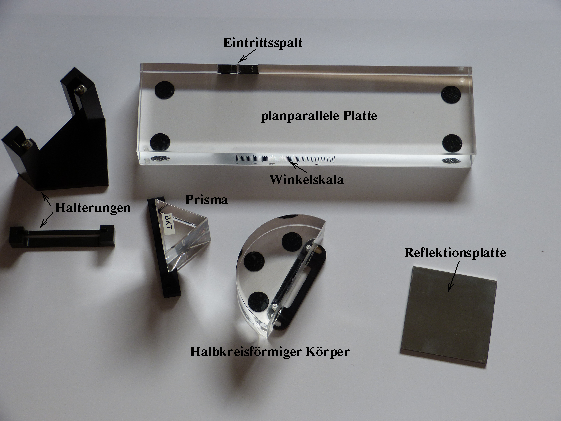
\includegraphics[width=\textwidth]{content/img/Abb_4.pdf}
      \caption{Blockschaltbild der verwendeten Messapparatur (mit im Text beschriebenen Änderungen). \cite{versuchsanleitung}}
      \label{fig:Aufbau}
    \end{figure}

    Die Eingangsspannung $U_\text{E}$ wird von einem Sinusgenerator
    mit einer Frequenz von $\SI{35}{\kilo\hertz}$ erzeugt,
    welche entsprechend als Durchlassfrequenz des Selektivverstärkers eingestellt wird.
    Der Sinusgenerator wird an die in \autoref{fig:Brückenschaltung} gezeigte Brückenschaltung angeschlossen,
    welche mit dem Selektivverstärker verbunden ist.
    Die in \autoref{fig:Aufbau} zu sehenden Verstärker vor und hinter dem Selektivverstärker werden hier nicht verwendet.
    Die Brückenspannung wird allerdings am Selektivverstärker 10-fach verstärkt.
    Der Selektivverstärker ist wiederum mit einem Spannungsmessgerät verbunden,
    welches übder diesen die Brückenspannung $U_\text{Br}$ misst.\\
    \\
    Zu Beginn wird die Gesamtverstärkung gemessen,
    indem die maximale Brückenspannung mit und ohne Verstärkung gemessen wird.\\
    Bei der Ausmessung der Proben wird nun so vorgegangen,
    dass zu Anfang die Brücke ohne eingefügte Probe abgeglichen wird.
    Dazu wird der variable Widerstand $R_3/R_4$ so eingestellt,
    dass $U_\text{Br}$ minimal wird.
    Es werden $U_\text{Br}$ und $R_3/R_4$ notiert.
    Anschließend wird die erste Probe,
    in diesem Fall $\ce{^{203}Dy}$,
    vorsichtig in eine der zylinderförmigen Spulen in der Brückenschaltung eingefügt.
    Die Brücke wird erneut abgeglichen und es werden $U_\text{Br}$ und $R_3/R_4$ notiert.
    % Dopplung: Mithilfe
    Mithilfe der Differenzen zwischen den Spannungen und Widerständen mit und ohne Probe
    kann aus den Gleichungen \eqref{eqn:SusU} und \eqref{eqn:SusR} nun
    die paramagnetische Suszeptibilität der $\ce{^{203}Dy}$-Probe berechnet werden.
    Die gesamte Messung für $\ce{^{203}Dy}$ wird dreimal ausgeführt.\\
    Für die zweite Probe $\ce{^{203}Nd}$ wird analog verfahren;
    auch diese Messung wird dreimal wiederholt.\\
    %\\
    Anschließend wird die Länge $l$ der beiden Proben jeweils dreimal ausgemessen,
    um später \hyperref[eqn:Q_real]{$Q_\text{real}$ berechnen zu können}.
